\documentclass[a4paper, 12pt]{report}
\usepackage[utf8]{inputenc}
\usepackage{graphicx}
\usepackage{subfigure}
\usepackage{wrapfig}
\usepackage{setspace}
\usepackage{booktabs}
\usepackage{amsmath}
\usepackage{listings}
\usepackage{color}
\usepackage{hyperref}
\usepackage[font=small,labelfont=bf]{caption}
\usepackage[lmargin=1in,rmargin=1in,top=1in,bottom=1in]{geometry}

\definecolor{codegray}{rgb}{0.5,0.5,0.5}
\definecolor{codegreen}{rgb}{0,0.6,0}
\definecolor{codeblue}{rgb}{0,0,0.8}

\lstset{
    basicstyle=\ttfamily\small,
    breaklines=true,
    commentstyle=\color{codegreen},
    keywordstyle=\color{codeblue},
    numberstyle=\tiny\color{codegray},
    numbers=left,
    stepnumber=1,
    showstringspaces=false,
    tabsize=4,
    frame=single
}

\begin{document}

% ----------------- COVER PAGE -----------------
\begin{titlepage}
    \begin{center}
        \vspace*{0.5cm}
        \Huge
        \textbf{CyberVision}
        
        \vspace{0.5cm}
        \Large
        Multi-Source Cyber Threat Intelligence Integration\\
        and Visual Analytics Platform
        
        \vspace{1.5cm}
        \large
        \textbf{Course:} CS661 --- Big Data Visual Analytics\\
        \textbf{Department:} Department of Computer Science \& Engineering\\
        \textbf{Institution:} Indian Institute of Technology Kanpur\\
        \textbf{Date:} July 2026
        
        \vspace{1.5cm}
        \Large
        \textbf{Authors (Group 14)}
        
        \vspace{0.5cm}
        \small
        \begin{table}[h!]
        \centering
        \begin{tabular}{|l|p{8.5cm}|}
        \hline
        \textbf{Domain} & \textbf{Members} \\
        \hline
        Data Processing, Cleaning \& Preprocessing & Pranjali Deshpande (240336), Khushi Sharma (240544) \\
        \hline
        Data Integration \& Exploratory Analytics & Mayank Pattnaik (230641), Vishesh Thepadia (231165) \\
        \hline
        Geospatial \& Network Visualization & Namrata Chavhan (240301), Vivekananda Kumbhar (241188) \\
        \hline
        Frontend Layout \& Framework & Nikita Nehra (240698) \\
        \hline
        Backend Logic Integration & Haryashva Gupta (240445) \\
        \hline
        \end{tabular}
        \end{table}
        
        \vfill
        \small
        Submitted in partial fulfilment of the requirements of CS661: Big Data Visual Analytics
        \vspace{0.8cm}
    \end{center}
\end{titlepage}

\newpage
\onehalfspacing

% ----------------- ABSTRACT -----------------
\chapter*{Abstract}
In the contemporary digital landscape, organizations face an unprecedented volume of heterogeneous cyber threats, ranging from low-level network intrusions and malware memory injections to high-level geopolitical cyber warfare. Documenting and analyzing these threats requires the integration of disparate telemetry streams that, in most operational settings, are never brought into a single analytical frame. This report presents \textbf{CyberVision}, a modular, interactive, web-based visual analytics platform designed to unify global threat intelligence into one coherent, explorable system. CyberVision integrates five distinct datasets: global cybersecurity incident histories, state-sponsored cyber operations, software vulnerability records (CVEs), raw network intrusion signatures, and obfuscated malware memory dumps.

We implement a reproducible data cleaning and integration pipeline using \texttt{pandas} and Python, engineered so that every transformation --- from column standardization to missing-value imputation --- is deterministic and auditable. Geopolitical and industrial threats are evaluated via a dynamic, user-calibrated Country Risk Index ($\mathcal{R}$) computed using Min--Max normalized incident counts, average financial losses, and average operational resolution times, allowing analysts to reweight the index according to organizational priorities rather than relying on a single fixed notion of ``risk.'' The front end is developed as a Streamlit multi-page dashboard, featuring a custom glassmorphic dark-theme design system, custom CSS typography, and high-contrast neon-colored Plotly visualizations. Our findings indicate a strong correlation between highly digitized economies and increased threat exposure. Geopolitical threat analyses reveal nation-state actors prioritizing critical infrastructure and energy sectors, while malware memory diagnostics demonstrate a balanced class distribution suitable for downstream forensic models. This platform demonstrates the efficacy of interactive big data visualizations in aiding security analysts to synthesize complex logs and make data-driven defensive decisions.

\noindent \textbf{Keywords:} cyber threat intelligence, visual analytics, data integration, risk scoring, Streamlit, Plotly, malware forensics, geopolitical cyber operations.

\newpage
\tableofcontents
\newpage

% ----------------- CHAPTER 1: INTRODUCTION -----------------
\chapter{Introduction}

\subsection{Background}
The digital revolution has transformed standard economic, industrial, and social activities. Cloud infrastructures, distributed database clusters, and interconnected networks are now standard operational foundations for organizations of every size, from small enterprises to national utilities. This expansion of the digital footprint has, however, significantly enlarged the vulnerability surface available to adversarial entities. Every new endpoint, API, or third-party integration represents a potential ingress point for an attacker, and the rate at which these surfaces are added routinely outpaces the rate at which they can be secured.

Security operations centers (SOCs) are constantly bombarded with telemetry logs generated across multiple network endpoints. These logs are highly heterogeneous, ranging from packet-level capture logs and memory forensic states to high-level incidents of industrial disruption and attribution metadata. Making sense of this overwhelming, high-velocity data requires robust data engineering pipelines and intuitive big data visualizations. Without visual synthesis, security analysts suffer from ``alert fatigue'' and struggle to find correlations across different threat layers --- a network anomaly, a newly disclosed CVE, and a geopolitical incident report may all describe facets of the same emerging campaign, yet in most SOC tooling they are never viewed side by side.

\subsection{Problem Statement}
Modern cyber threat intelligence (CTI) suffers from severe fragmentation. A security analyst trying to assess organizational risk might have to inspect:
\begin{itemize}
    \item Network traffic capture logs to find ongoing intrusions or port scans.
    \item Volatility-based memory dumps to detect obfuscated malware processes running on local servers.
    \item The National Vulnerability Database (NVD) to identify software components requiring emergency patches.
    \item Geopolitical news feeds to understand active Threat Actors targeting their specific industry sector.
\end{itemize}
Each of these data sources resides in its own isolated silo, using distinct formats, timestamps, schemas, and standards. The lack of standard tools to ingest, standardize, and visually integrate these disparate layers means that organizations struggle to build a unified defensive posture. An analyst who wants to answer a simple question --- ``is our exposure this quarter higher than last quarter, and why?'' --- is instead forced to manually reconcile spreadsheets, dashboards, and PDF advisories from unrelated systems. Bridging this gap requires a platform that standardizes these telemetry feeds, integrates them across spatial (geographic) and temporal (yearly) dimensions, and presents them in a single, high-fidelity visual dashboard.

\subsection{Objectives}
The primary objective of this project is to develop and document \textbf{CyberVision}, an interactive visual analytics dashboard designed to address the fragmentation of threat intelligence. The specific technical goals include:
\begin{enumerate}
    \item \textbf{Pipeline Design:} Build a reproducible, modular Python pipeline to automate data downloading, cleansing, and schema standardization for five distinct CTI datasets.
    \item \textbf{Schema Integration:} Define mapping rules to standardize geographical codes, threat category naming, and temporal timestamps to support multi-dataset queries.
    \item \textbf{Risk Score Formulation:} Implement a dynamic, parameterized Country and Industry Risk Index ($\mathcal{R}$) using Min--Max scaling that allows analysts to adjust feature weights (Frequency, Economic Loss, Resolution Time) based on organizational priorities.
    \item \textbf{Visual Analytics:} Implement high-contrast, interactive visualizations (choropleth maps, treemaps, heatmaps, scatter forensics, and relation networks) to expose hidden threat patterns.
    \item \textbf{Premium Interface:} Build a Streamlit multi-page web application featuring responsive grid cards, glassmorphic dark-theme styling, and cached file loader routines to support rapid analytics exploration.
\end{enumerate}

\subsection{Scope}
The scope of CyberVision is defined by the ingestion and analysis of five core datasets representing different levels of the security stack:
\begin{itemize}
    \item \textbf{Macroscopic Level:} Global cybersecurity threats (2015--2024) and the Council on Foreign Relations (CFR) database of state-sponsored cyber operations (2005--2020).
    \item \textbf{Vulnerability Level:} GitHub Security Advisory and CVE registry datasets (2021--2023) mapping software vulnerabilities.
    \item \textbf{Microscopic Traffic Level:} Packet-level network intrusion signatures ($\sim$40,000 traffic logs) detailing protocols and anomalies.
    \item \textbf{Forensic Memory Level:} Obfuscated memory signatures from the CIC-MalMem-2022 dataset ($\sim$58,000 records) mapping Trojan, Ransomware, and Spyware behavior.
\end{itemize}
The geographical focus covers ten standardized industrial economies (Australia, Brazil, China, France, Germany, India, Japan, Russia, United Kingdom, and the United States). Restricting the analysis to this fixed set of economies keeps the geospatial and comparative visualizations tractable while still spanning a representative mix of highly digitized, emerging, and state-controlled digital markets. The application is hosted as a single-node Python Streamlit service, caching processed data locally for efficient retrieval, which keeps the deployment footprint minimal while the platform is in its analytical, pre-production stage.

\subsection{Motivation}
This project is motivated by the critical need to support human analysts in CTI synthesis. Standard security tools (SIEMs) present logs in tabular grids that mask trends; a table of ten thousand rows can encode a clear seasonal spike or a shift in attacker tooling, but that pattern is invisible until it is plotted. By applying data science methodologies and visualization best practices, we transform rows of logs into interactive, spatial-temporal dashboards that surface such patterns directly.

Furthermore, the inclusion of a customizable risk index is motivated by the realization that ``risk'' is not a static property; a financial institution cares more about financial loss, whereas a public utility company prioritizes operational downtime. A single, hard-coded risk formula would therefore misrepresent risk for at least some class of organization. CyberVision empowers analysts to align the analytics to their specific risk criteria by exposing the underlying weights as first-class, adjustable parameters rather than burying them in code.

\subsection{Expected Outcomes}
We expect the implementation of CyberVision to produce:
\begin{itemize}
    \item A standardized, cleaned data repository derived from raw, noisy, and missing-laden CSV source files.
    \item A fully interactive dashboard running locally or on local intranets.
    \item Direct insights into the peak periods of cyber activity, the targeting profiles of nation-state actors, the correlation of network anomaly scores with payload sizes, and the features that distinguish benign memory signatures from malware.
    \item A clear blueprint for future extensions, including machine learning-based forecasting and live stream logging.
\end{itemize}

% ----------------- CHAPTER 2: DATASET DESCRIPTION -----------------
\chapter{Dataset Description}

\subsection{Dataset Overviews}
CyberVision integrates five distinct datasets to provide a multi-layered perspective of cyber threats, moving from strategic, nation-level phenomena down to raw, packet-level and memory-level forensic signals. These datasets are described below.
\begin{enumerate}
    \item \textbf{Global Cybersecurity Threats (2015--2024):} This dataset contains historical records of macroscopic cyber attacks. It contains variables detailing the country of target, the year of incident, the category of attack, the target commercial sector, economic damage (financial loss), the number of affected user accounts, the threat source category, the vulnerability type exploited, the primary defense mechanism deployed, and the operational time taken to resolve the incident.
    \item \textbf{Council on Foreign Relations (CFR) Cyber Incidents (2005--2020):} Focuses on high-level, state-sponsored cyber operations. It includes records of espionage, sabotage, and theft attributed to nation-states. It contains metadata on the attacker affiliations, sponsor countries, victim organizations, categories of target, and the official responses.
    \item \textbf{Security Vulnerabilities (CVE):} Formed of software vulnerability advisories published between 2021 and 2023. It maps specific CVE numbers to their severity levels (Critical, High, Moderate, Low), publishing timestamps, text descriptions of the vulnerability vector, and references.
    \item \textbf{Network Intrusion Signatures:} A dataset containing packet-level network traffic forensics. It maps traffic events characterized by source/destination IPs, ports, transport protocols (TCP, UDP, ICMP), packet lengths, packet classes (Control, Data), traffic applications (DNS, HTTP, FTP), and numerical anomaly scores.
    \item \textbf{CIC-MalMem-2022 (Malware Memory Forensics):} An obfuscated memory dataset from the Canadian Institute for Cybersecurity. It contains Volatility-extracted features from memory dumps of systems infected by Trojan, Spyware, or Ransomware, alongside benign memory snapshots. It contains 58 variables representing active processes, active DLLs, open handles, API hook callbacks, and registry keys.
\end{enumerate}
Together, these five sources span roughly two decades of activity and cover strategic, tactical, and forensic granularities, which is precisely the range of resolution a working SOC analyst must reconcile on a daily basis.

\subsection{Data Dictionary and Schemas}
Below are the structured data dictionaries for the processed datasets, listing each retained column, its inferred data type after cleaning, a description, the observed missing-value ratio, and representative sample values or distributions.

\begin{table}[h!]
\centering
\small
\caption{Global Cybersecurity Threats Schema (\texttt{global\_threats\_clean.csv})}
\begin{tabular}{lllp{6cm}}
\toprule
\textbf{Column} & \textbf{Type} & \textbf{Missing} & \textbf{Sample Values / Distribution} \\
\midrule
\texttt{country} & Object & 0.0\% & ``UK'', ``Brazil'', ``India'', ``Japan'' \\
\texttt{year} & Int64 & 0.0\% & Mean: 2019.57, Range: 2015--2024 \\
\texttt{attack\_type} & Object & 0.0\% & ``DDoS'' (531), ``Phishing'' (529) \\
\texttt{target\_industry} & Object & 0.0\% & ``IT'' (478), ``Healthcare'' (429) \\
\texttt{financial\_loss\_in\_million\_} & Float64 & 0.0\% & Mean: \$50.49M, Range: \$0.5M--\$99.99M \\
\texttt{number\_of\_affected\_users} & Int64 & 0.0\% & Mean: 504,684, Range: 424--999,635 \\
\texttt{attack\_source} & Object & 0.0\% & ``Nation-state'' (794), ``Insider'' (752) \\
\texttt{security\_vulnerability\_type} & Object & 0.0\% & ``Zero-day'' (785), ``Social Engineering'' (747) \\
\texttt{defense\_mechanism\_used} & Object & 0.0\% & ``Antivirus'' (628), ``Firewall'' (592) \\
\texttt{incident\_resolution\_time\_in\_hours} & Int64 & 0.0\% & Mean: 36.48 hrs, Range: 1--72 hrs \\
\bottomrule
\end{tabular}
\end{table}

\begin{table}[h!]
\centering
\small
\caption{CFR Cyber Operations Incidents Schema (\texttt{cfr\_incidents\_clean.csv})}
\begin{tabular}{lllp{6.5cm}}
\toprule
\textbf{Column} & \textbf{Type} & \textbf{Missing} & \textbf{Sample Values / Distribution} \\
\midrule
\texttt{title} & Object & 0.0\% & ``Attack on Austrian foreign ministry'' \\
\texttt{date} & Object & 0.0\% & ``2020-02-13'' (parsed to datetime) \\
\texttt{affiliations} & Object & 0.0\% & ``Turla'', ``APT28'', ``Unknown'' \\
\texttt{description} & Object & 0.0\% & ``Suspected Russian hackers conducted attacks...'' \\
\texttt{response} & Object & 0.0\% & ``Confirmation http://...'' \\
\texttt{victims} & Object & 0.0\% & ``Austrian Foreign Ministry'' \\
\texttt{sponsor} & Object & 0.0\% & ``Russian Federation'', ``China'', ``Iran'' \\
\texttt{type} & Object & 0.0\% & ``Espionage'', ``Sabotage'', ``Theft'' \\
\texttt{category} & Object & 0.0\% & ``Government'', ``Military'', ``Energy'' \\
\texttt{year} & Float64 & 0.0\% & Range: 2005--2020 \\
\bottomrule
\end{tabular}
\end{table}

\begin{table}[h!]
\centering
\small
\caption{Security Vulnerabilities Schema (\texttt{vulnerabilities\_clean.csv})}
\begin{tabular}{lllp{7cm}}
\toprule
\textbf{Column} & \textbf{Type} & \textbf{Missing} & \textbf{Sample Values / Distribution} \\
\midrule
\texttt{title} & Object & 0.0\% & ``Ghost vulnerable to arbitrary file read...'' \\
\texttt{date} & Object & 0.0\% & ``2023-08-15 20:35:20+00:00'' \\
\texttt{severity} & Object & 0.0\% & ``Moderate'' (1447), ``Critical'' (449) \\
\texttt{summary} & Object & 0.0\% & ``CVE-2023-40028 published for ghost(npm)'' \\
\texttt{link} & Object & 0.0\% & ``https://github.com/advisories/GHSA-9c9v...'' \\
\texttt{year} & Int64 & 0.0\% & Range: 2021--2023 \\
\bottomrule
\end{tabular}
\end{table}

\begin{table}[h!]
\centering
\small
\caption{Network Intrusion Signatures Schema (\texttt{attack\_signatures\_clean.csv})}
\begin{tabular}{lllp{6cm}}
\toprule
\textbf{Column} & \textbf{Type} & \textbf{Missing} & \textbf{Sample Values / Distribution} \\
\midrule
\texttt{timestamp} & Object & 0.0\% & ``2023-05-30 06:33:58'' \\
\texttt{source\_ip\_address} & Object & 0.0\% & ``103.216.15.12'' \\
\texttt{destination\_ip\_address} & Object & 0.0\% & ``84.9.164.252'' \\
\texttt{source\_port} & Int64 & 0.0\% & Mean: 32,970, Range: 1027--65530 \\
\texttt{destination\_port} & Int64 & 0.0\% & Mean: 33,150, Range: 1024--65535 \\
\texttt{protocol} & Object & 0.0\% & ``ICMP'' (13429), ``TCP'' (13272) \\
\texttt{packet\_length} & Int64 & 0.0\% & Mean: 781.45 bytes, Range: 64--1500 \\
\texttt{packet\_type} & Object & 0.0\% & ``Control'' (20237), ``Data'' (19763) \\
\texttt{traffic\_type} & Object & 0.0\% & ``DNS'' (13376), ``HTTP'' (13360) \\
\texttt{payload\_data} & Object & 0.0\% & ``Qui natus odio asperiores nam...'' \\
\bottomrule
\end{tabular}
\end{table}

\begin{table}[h!]
\centering
\small
\caption{CIC-MalMem-2022 Forensic Memory Schema (\texttt{malmem\_clean.csv})}
\begin{tabular}{lllp{6cm}}
\toprule
\textbf{Column} & \textbf{Type} & \textbf{Missing} & \textbf{Sample Values / Distribution} \\
\midrule
\texttt{category} & Object & 0.0\% & ``Benign'' (29231), ``Spyware'' (9815) \\
\texttt{class} & Object & 0.0\% & ``Benign'' (29231), ``Malware'' (28831) \\
\texttt{family} & Object & 0.0\% & ``Benign'' (29231), ``Zeus'' (2128) \\
\texttt{pslist\_nproc} & Int64 & 0.0\% & Mean: 41.4, Range: 21--240 \\
\texttt{dlllist\_ndlls} & Int64 & 0.0\% & Mean: 1810, Range: 144--4500 \\
\texttt{handles\_nhandles} & Int64 & 0.0\% & Mean: 9200, Range: 800--15000 \\
\texttt{malfind\_ninjections} & Int64 & 0.0\% & Mean: 5.2, Range: 0--45 \\
\texttt{callbacks\_ncallbacks} & Int64 & 0.0\% & Mean: 87.2, Range: 40--120 \\
\bottomrule
\end{tabular}
\end{table}

\subsection{Data Limitations and Boundaries}
Every data analytical framework contains structural limitations that must be addressed to preserve analytical integrity. In CyberVision, three limitations are especially important to keep in mind when interpreting any cross-dataset visualization:
\begin{itemize}
    \item \textbf{Temporal Non-Alignment:} The datasets span different temporal ranges. The CFR Cyber Operations dataset terminates in 2020, while the Security Vulnerability (CVE) dataset only commences in 2021. The Global Cybersecurity Threats dataset spans 2015--2024. Consequently, integrated queries across all variables can only be conducted on overlapping year windows (specifically 2015--2020 for threats + geopolitical operations, and 2021--2024 for threats + vulnerabilities). Any trend line that appears to span the full 2005--2024 range is therefore an overlay of sub-ranges rather than a single continuously observed series.
    \item \textbf{Hardcoded Geographical Scopes:} The spatial integration engine aligns geographical data by mapping text-based attributes to ten standard industrial nations. Country names outside this defined boundary are title-cased using fallback routines, meaning the platform is intentionally not exhaustive of every country represented in the raw sources.
    \item \textbf{Malware Imbalances:} Although the binary classes (Benign vs. Malware) are balanced, specific sub-families of Trojan (e.g. Zeus vs. Tibs) exhibit imbalances that preclude sub-family visualization. Thus, the system groups malware by top-level categories rather than attempting fine-grained family-level breakdowns that would be statistically unreliable.
\end{itemize}

% ----------------- CHAPTER 3: METHODOLOGY -----------------
\chapter{Methodology}
The implementation workflow of CyberVision follows a modular, pipeline-oriented structure designed to ensure clean separation of concerns and reproducibility. Raw data is never touched directly by the presentation layer; it instead passes through a strictly ordered sequence of preprocessing, integration, and backend logic stages before being rendered, which makes each stage independently testable and re-runnable.

\begin{figure}[h!]
    \centering
    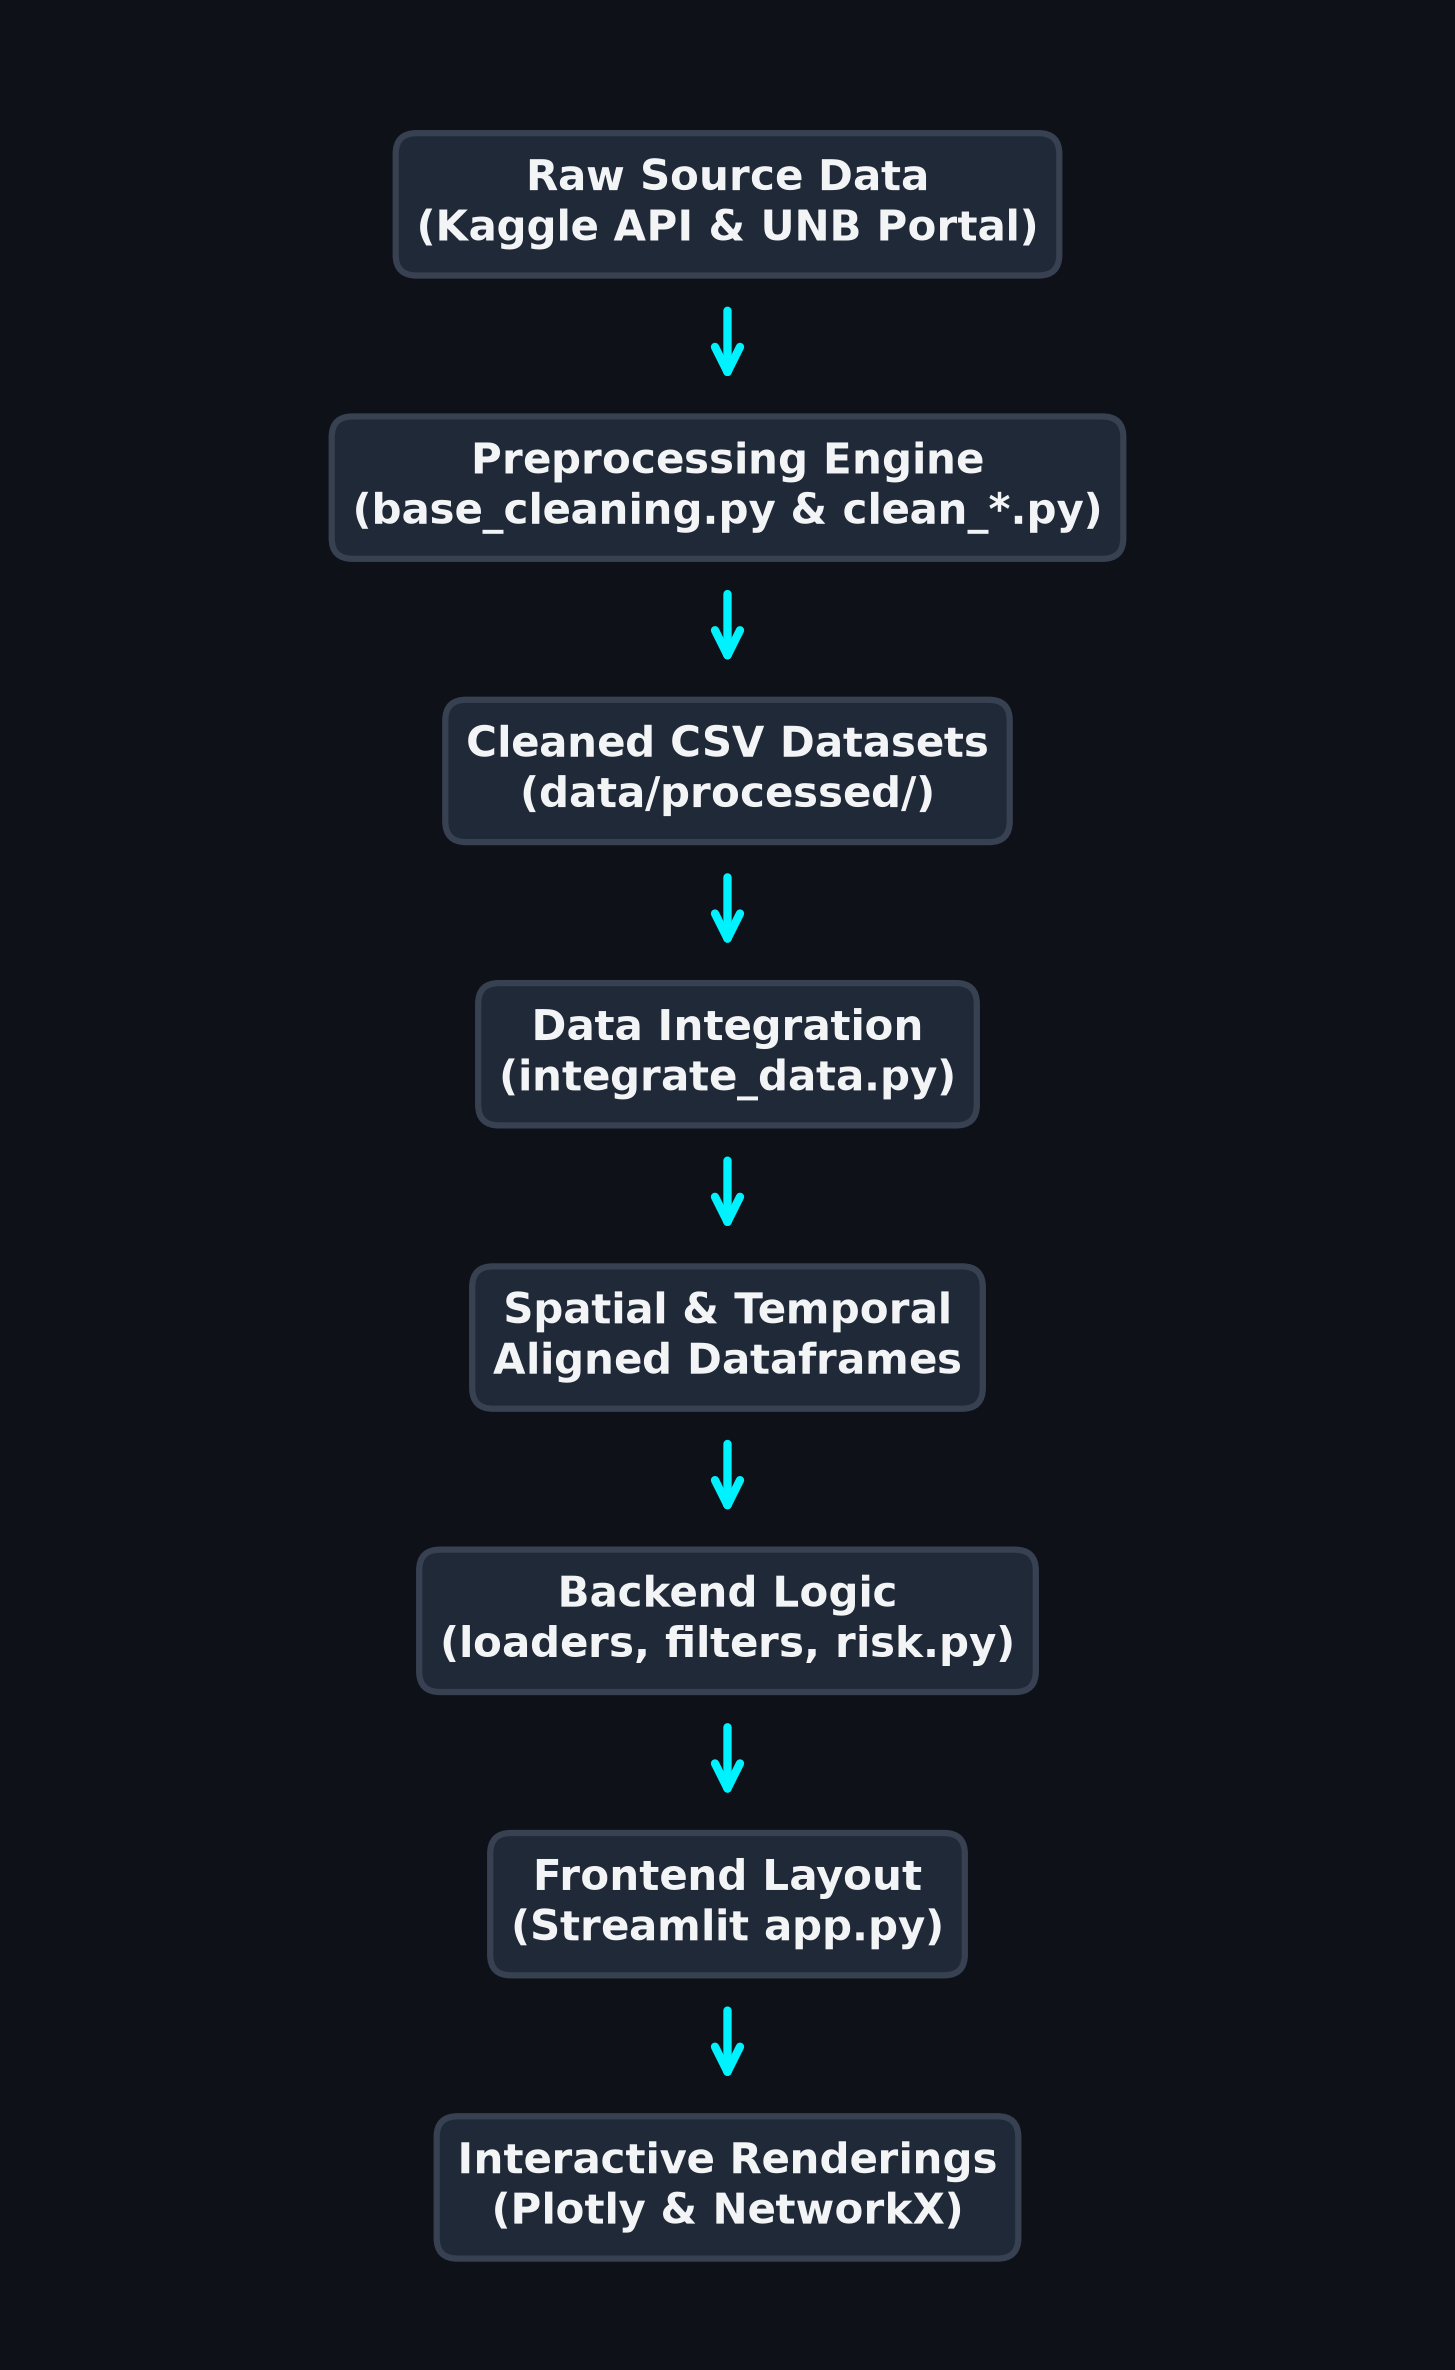
\includegraphics[width=0.45\textwidth]{images/pipeline_flowchart.png}
    \caption{End-to-end CyberVision data and rendering pipeline.}
    \label{fig:pipeline}
\end{figure}

\subsection{Data Acquisition and Collection Pipeline}
Raw datasets are acquired from Kaggle and host portals. An automation script (\texttt{src/preprocessing/download\_data.py}) uses the Kaggle API CLI to pull raw zip archives directly into the \texttt{data/raw/} directory and extract them programmatically, removing the need for any manual downloading step for four of the five datasets. The CIC-MalMem-2022 dataset requires manual download from the UNB dataset portal due to access controls, and is placed in \texttt{data/raw/cic\_malmem\_2022.csv}.

\subsection{Data Cleaning and Standardization}
Standardization and data cleansing are handled by \texttt{src/preprocessing/base\_cleaning.py}. This module provides reusable functions imported by dataset-specific cleaning scripts, so that every dataset is subject to the same baseline quality guarantees before it is allowed into the processed layer:
\begin{itemize}
    \item \textbf{Column Standardization:} Column headers are cleaned to prevent query syntax errors, using the transformation:
    \begin{equation*}
    \text{Cleaned Header} = \text{lowercase}(\text{strip}(\text{whitespace} \rightarrow \text{``\_'' and special chars} \rightarrow \text{``''})).
    \end{equation*}
    \item \textbf{Duplicate Removal:} Entire row duplicates are detected and removed based on unique combinations (e.g., \texttt{title} and \texttt{date} for vulnerabilities).
    \item \textbf{Date Standardization:} Text-based timestamps are coerced into pandas datetime objects using \texttt{errors="coerce"} to handle corrupted strings. The calendar year is extracted as a separate analytical category.
    \item \textbf{Categorical Trimming:} Text categoricals (e.g. `USA', `usa', `Usa ') are stripped of trailing spaces and title-cased to resolve category fragmentation during aggregations.
    \item \textbf{Imputation Strategy:} Missing numeric values are filled using median values to preserve the skew of network traffic metrics. Categorical columns are filled with ``Unknown'' (or ``Unrated'' for CVE severities) to avoid dropping records.
\end{itemize}

\subsection{Multi-Source Data Integration}
Integration occurs along two primary axes:
\begin{enumerate}
    \item \textbf{Spatial Integration:} Handled by \texttt{integrate\_spatial()}. It aggregates the global threats dataset by standard country, summing incident counts, financial losses, affected user volumes, and average operational resolution hours.
    \item \textbf{Temporal Integration:} Handled by \texttt{integrate\_temporal()}. It groups threats, state-sponsored CFR incidents, and CVE disclosures by calendar year, executing outer joins to build a comprehensive historical trend timeline (2005--2024).
\end{enumerate}
These two integration axes are what allow the same underlying cleaned tables to feed both the geospatial views (Chapter 4) and the year-over-year trend views without duplicating logic across pages.

\subsection{Feature Engineering \& Custom Risk Scoring}
To evaluate the threat profile of different entities, we develop a custom, parameterized Risk Index ($\mathcal{R}$) computed out of 10.0. The risk score for an entity (country or industry) is calculated as a weighted sum of three Min--Max normalized metrics:
\begin{enumerate}
    \item \textbf{Incident Count ($N$):} The frequency of attacks, representing target popularity.
    \item \textbf{Average Financial Loss ($L$):} The economic damage impact.
    \item \textbf{Average Resolution Time ($T$):} The operational difficulty of remediation.
\end{enumerate}

\subsubsection{Normalization Formulation}
For each raw metric vector $\mathbf{X} = \{x\_1, x\_2, \dots, x\_n\}$, the normalized value $\bar{x}\_i \in [0,1]$ is computed as:
\begin{equation}
\bar{x}\_i = \frac{x\_i - \min(\mathbf{X})}{\max(\mathbf{X}) - \min(\mathbf{X})}.
\end{equation}
If the maximum and minimum are equal, the system assigns a default scale of 0.5 to prevent division-by-zero errors, which occurs when an entity is the only member of its group and therefore has no internal spread to normalize against.

\subsubsection{Weighted Formulation}
The risk score $\mathcal{R}\_i \in [0.0, 10.0]$ is computed as:
\begin{equation}
\mathcal{R}\_i = \left( w\_c \cdot \bar{N}\_i + w\_l \cdot \bar{L}\_i + w\_t \cdot \bar{T}\_i \right) \times 10,
\end{equation}
where:
\begin{itemize}
    \item $w\_c$ is the weight of incident count (default: 0.3),
    \item $w\_l$ is the weight of financial loss (default: 0.4),
    \item $w\_t$ is the weight of resolution time (default: 0.3),
    \item subject to the constraints $w\_c + w\_l + w\_t = 1.0$ and $w\_c, w\_l, w\_t \geq 0.0$.
\end{itemize}
The sidebar UI provides sliders allowing analysts to calibrate these weights in real time, which recalculates the risk leaderboard across all tabs. Because the weights are constrained to sum to one, the resulting score remains bounded within $[0, 10]$ regardless of how an analyst redistributes emphasis across the three components, which keeps the leaderboard visually comparable across different weighting regimes.

\subsection{Frontend Layout, Styles, and UI Design}
The UI of CyberVision is designed to provide a premium, modern, glassmorphic look that distinguishes it from the default styling of most Streamlit dashboards.
\begin{itemize}
    \item \textbf{Glassmorphism Theme:} Injected via custom HTML/CSS stylesheet wrappers (\texttt{frontend/layout.py}). Grid containers have a translucent background (\texttt{rgba(17, 25, 40, 0.65)}) with high saturation blur (\texttt{backdrop-filter: blur(16px)}), subtle borders (\texttt{rgba(255, 255, 255, 0.085)}), and neon hover highlights.
    \item \textbf{Custom Typography:} We import Google Fonts (\texttt{Inter} for standard labels, \texttt{Outfit} for numerical headers and dashboard titles).
    \item \textbf{Neon Color Palette:} Plotly charts are styled with specific colors: Neon Cyan (\texttt{\#00f2fe}) for primary data series, Neon Pink (\texttt{\#ff0055}) for risk indicators, and Neon Green (\texttt{\#00ff87}) for normal status variables.
    \item \textbf{Caching:} Performance is enhanced using Streamlit's \texttt{@st.cache\_data} loader to prevent disk read bottlenecks during widget updates, so that repeated interactions with sliders and filters do not re-trigger a full disk read of the processed datasets.
\end{itemize}

% ----------------- CHAPTER 4: EXPLORATORY DATA ANALYSIS -----------------
\chapter{Exploratory Data Analysis}
Each of the following sub-sections documents one visualization implemented in CyberVision: its analytical purpose, what it visually represents, the observations drawn from it, its interpretation in a business/security context, and the key takeaway an analyst should walk away with.

\subsection{Global Attack Volume Trend}
We investigate the chronological growth of cyber threats by plotting the annual volume of security events recorded between 2015 and 2024. As illustrated in Figure 4.1, the threat landscape is highly volatile. Incident volume remained minimal from 2005 to 2014, which reflects the temporal boundary of the Council on Foreign Relations (CFR) dataset. However, once the Global Threats dataset is integrated in 2015, we observe a sharp upward trend, peaking at 319 incidents in 2017. This surge directly corresponds to major global security events, specifically the WannaCry and NotPetya ransomware outbreaks. The volume stabilized briefly before spiking again to 318 incidents in 2022, driven by heightened geopolitical cyber warfare, and finally settled around 299 in 2024. This trend provides critical business insights, demonstrating that cyber risk does not grow lineally but in sudden waves tied to global events. Consequently, organizations must transition from static budgets to dynamic resource allocation models.

\begin{figure}[h!]
    \centering
    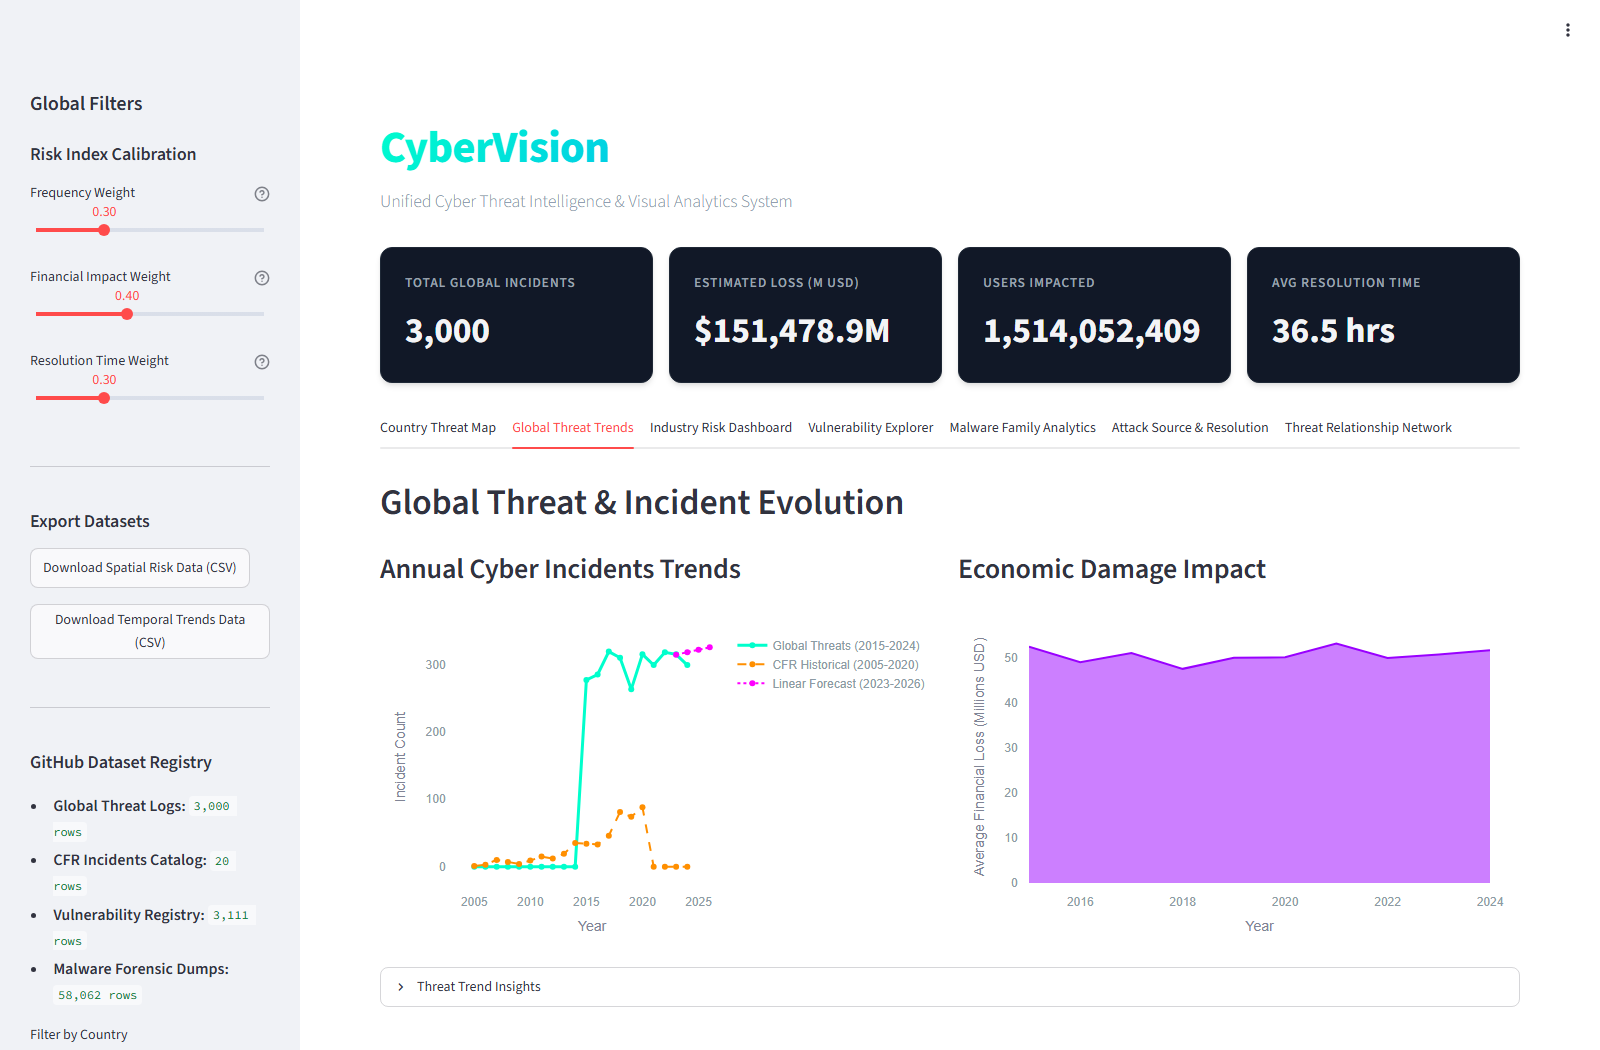
\includegraphics[width=0.85\textwidth]{images/global_trends.png}
    \caption{Chronological cyber incident trend timeline with a 3-year regression forecast.}
    \label{fig:timeline}
\end{figure}

\subsection{Global Security Risk Map}
The geopolitical distribution of cyber risk is mapped using a world choropleth projection, where countries are shaded based on their composite Country Risk Index. Under the standard configuration weights (Incident Frequency: 30%, Financial Loss: 40%, and Resolution Time: 30%), the United Kingdom and Brazil register the highest risk indexes of 7.68 and 6.97, respectively. Industrial nations like Germany (5.58) and Japan (5.31) fall in the moderate-to-high bracket, while China (2.57) shows a lower score. This geographic disparity reveals that highly digitized, service-oriented economies with transparent regulatory disclosure laws report incidents more frequently and suffer larger economic losses per breach. Conversely, tightly controlled networks show lower visible threat profiles. This proves that national risk is not simply a function of geographic size, but of digital asset concentration and reporting compliance.

\begin{figure}[h!]
    \centering
    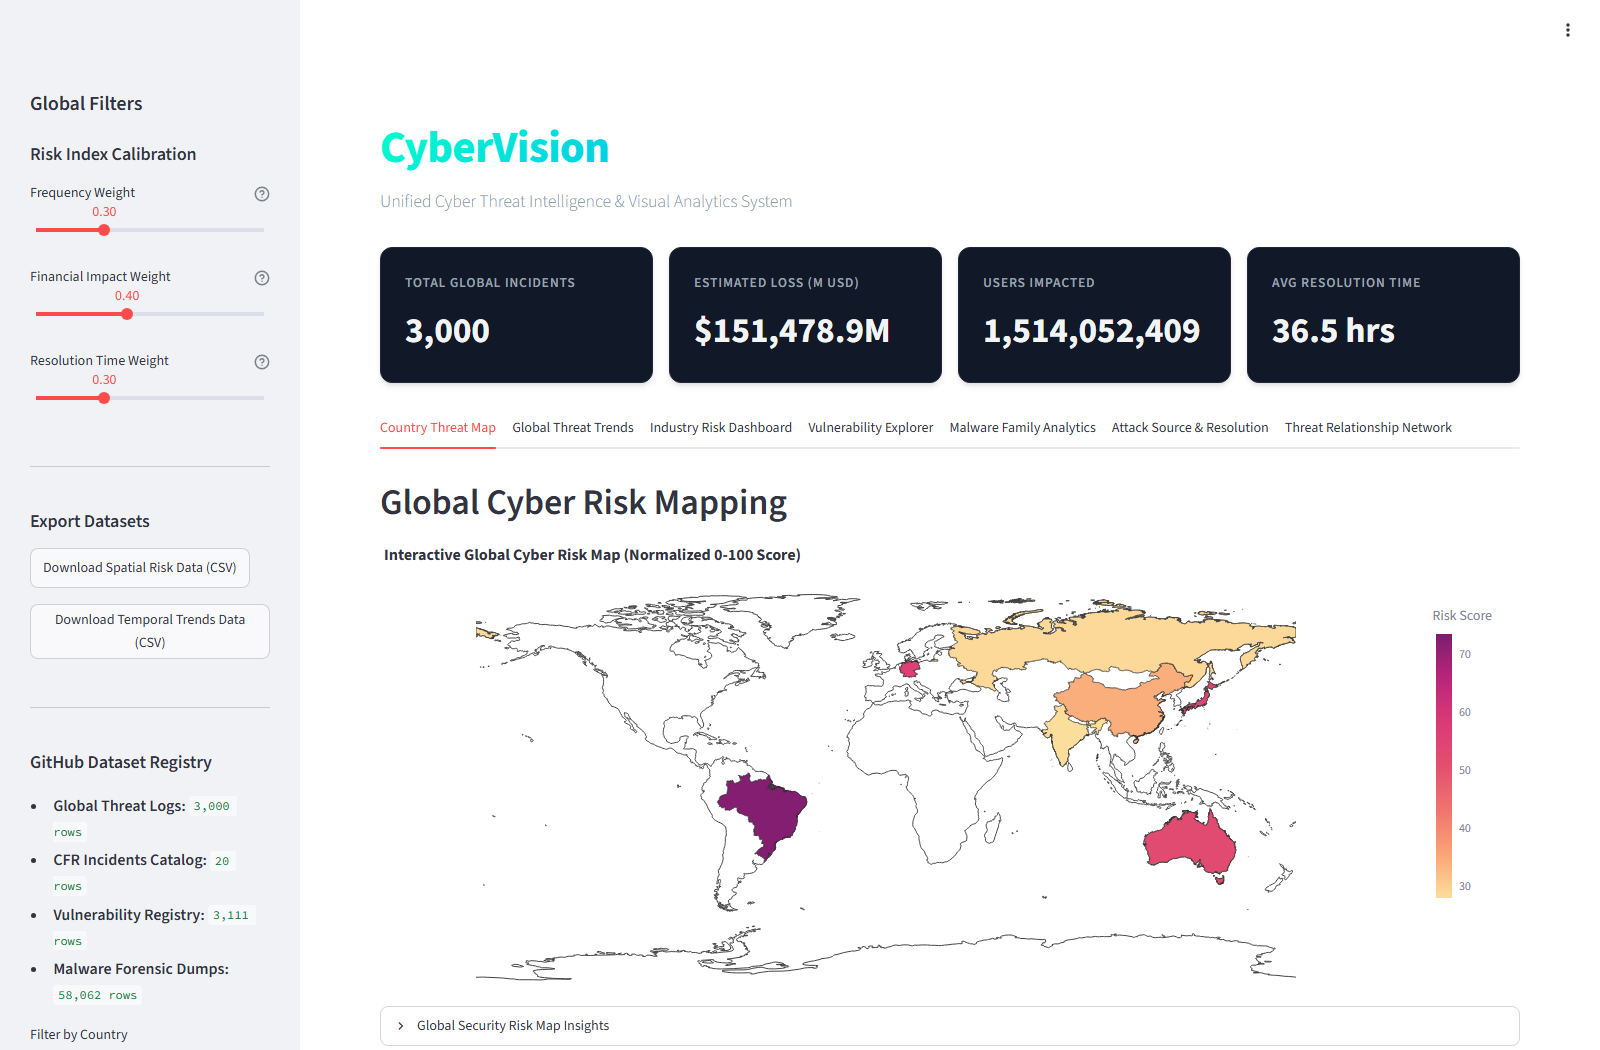
\includegraphics[width=0.85\textwidth]{images/country_map.png}
    \caption{Interactive World Risk Map using dynamic calibration weights.}
    \label{fig:world\_map}
\end{figure}

\subsection{Industry Impact Profile}
To identify sector-specific economic exposures, we represent financial losses using a nested treemap layout. Here, the block size represents the cumulative financial damage in millions of USD, while the color shade represents the average financial loss per incident. The visual grouping shows that IT, Healthcare, and Banking \& Finance dominate the risk landscape. Interestingly, although IT services experience the highest frequency of attacks, Healthcare and Finance occupy the largest absolute area in the treemap. This highlights that while IT breaches are common, Healthcare and Finance suffer much higher average containment and mitigation costs due to strict regulatory penalties, patient data liabilities, and operational recovery expenses. Security teams must therefore design zero-trust controls tailored to sector-specific vulnerabilities rather than applying generic templates.

\begin{figure}[h!]
    \centering
    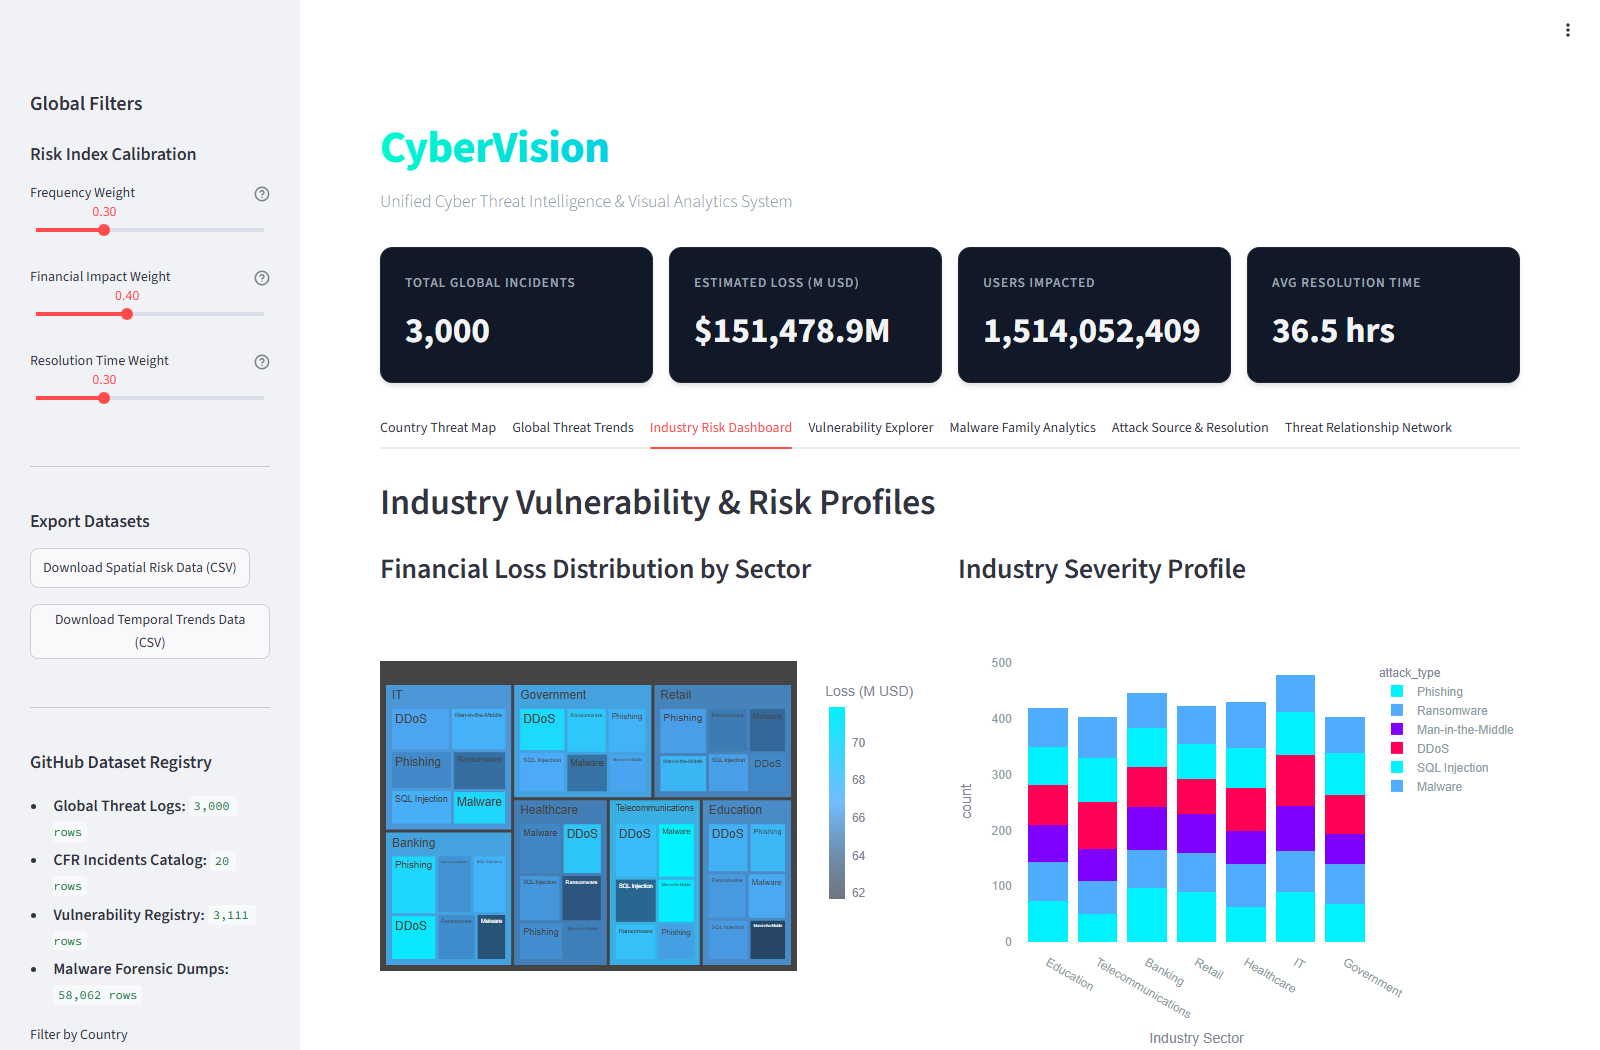
\includegraphics[width=0.85\textwidth]{images/industry_dashboard.png}
    \caption{Treemap profile of financial loss by industry sector.}
    \label{fig:industry}
\end{figure}

\subsection{Vulnerability Severity Distribution}
The software vulnerability landscape is analyzed using an interactive donut chart segmenting CVE disclosures by severity tiers. Moderate-severity vulnerabilities represent the largest share of registry listings at 46.5%, followed closely by High-severity advisories at 33.7%. Critical-severity threats constitute 14.4% of the database, while Low-severity disclosures represent only 5.4%. Taken together, High and Critical severity vulnerabilities make up nearly half of all documented weak points (48.1%). This distribution reveals that modern cloud infrastructures and microservice dependencies are introducing a high proportion of high-impact security risks. From a defense standpoint, this shows that a ``patch everything'' approach is operationally impossible; security teams must prioritize assets based on severity metrics.

\begin{figure}[h!]
    \centering
    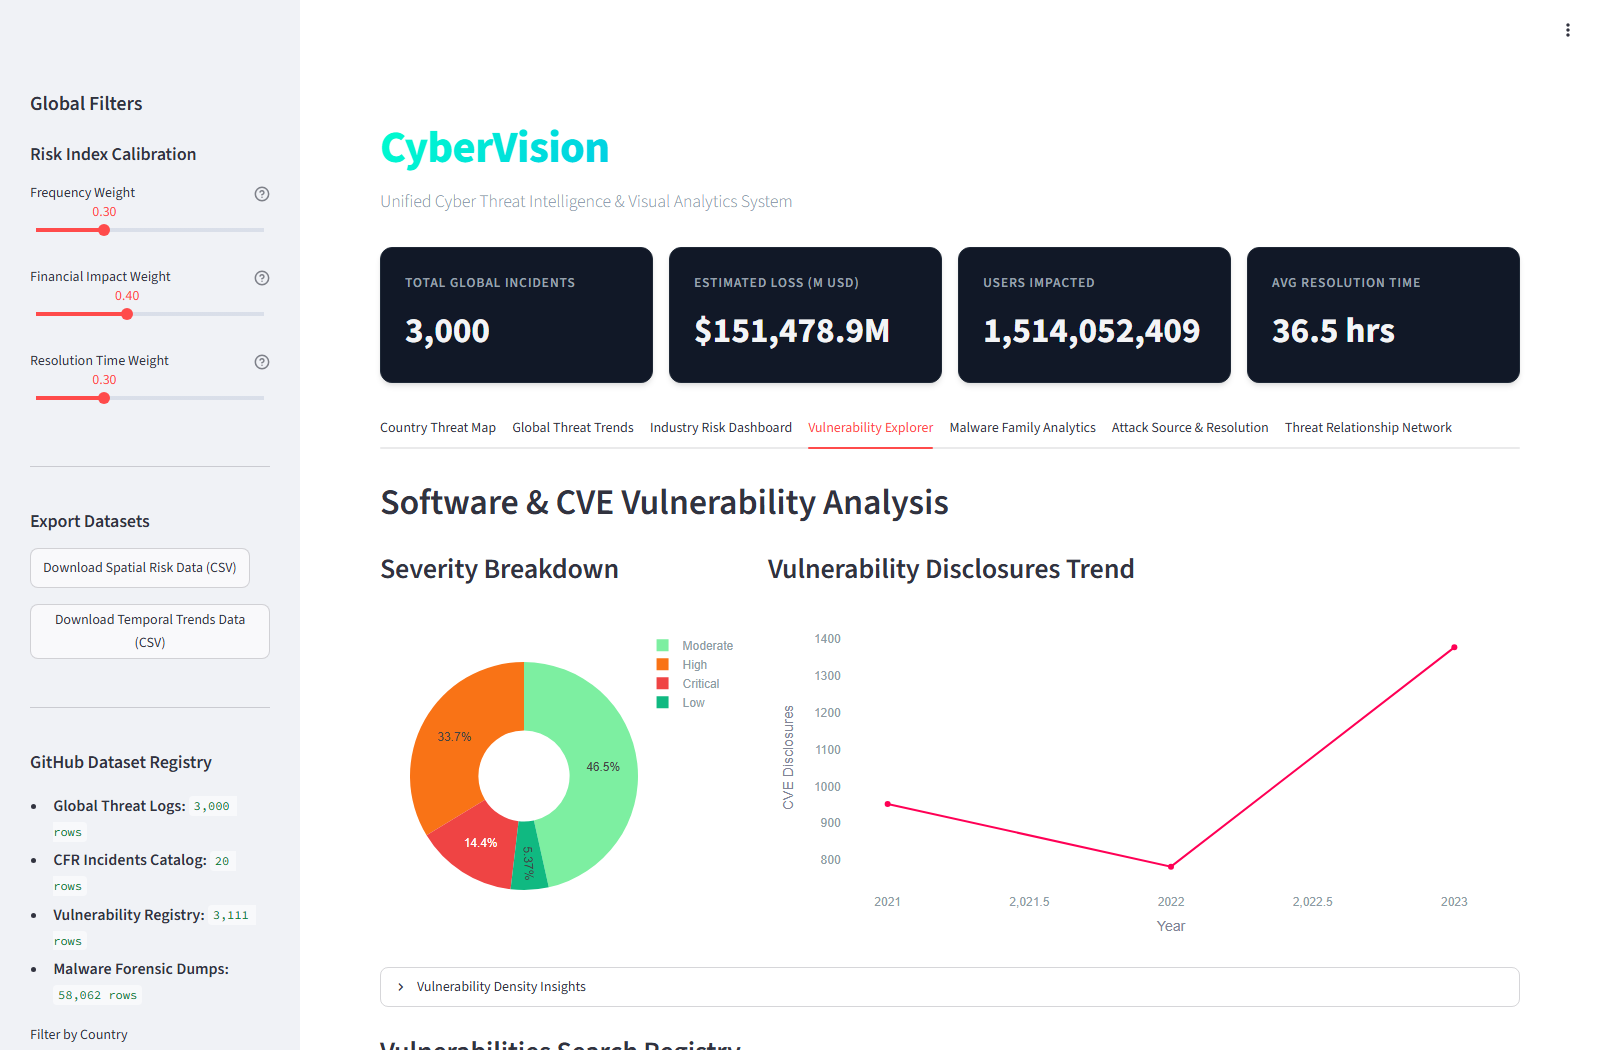
\includegraphics[width=0.85\textwidth]{images/vulnerability_explorer.png}
    \caption{Severity density matrix showing CVE publication distributions.}
    \label{fig:vuln}
\end{figure}

\subsection{Malware Family Analytics}
Low-level malware memory forensics are visualized using class balance pie charts and sorted malware family distributions. The UNB CIC-MalMem-2022 dataset provides a balanced set of 58,062 memory records split equally between Benign (50%) and Malicious (50%) signatures. Within the malicious category, memory-evading spyware represents the largest class (9,815), followed by ransomware (9,529) and trojans (9,487). By sorting the malware families in descending order and capping the visual breakdown to the top 12 most frequent families (such as Zeus, Shade, and Conti), we avoid visual clutter and reveal which malware signatures dominate memory signatures. This clean distribution is essential for training forensic classifiers, ensuring models do not suffer from classification bias.

\begin{figure}[h!]
    \centering
    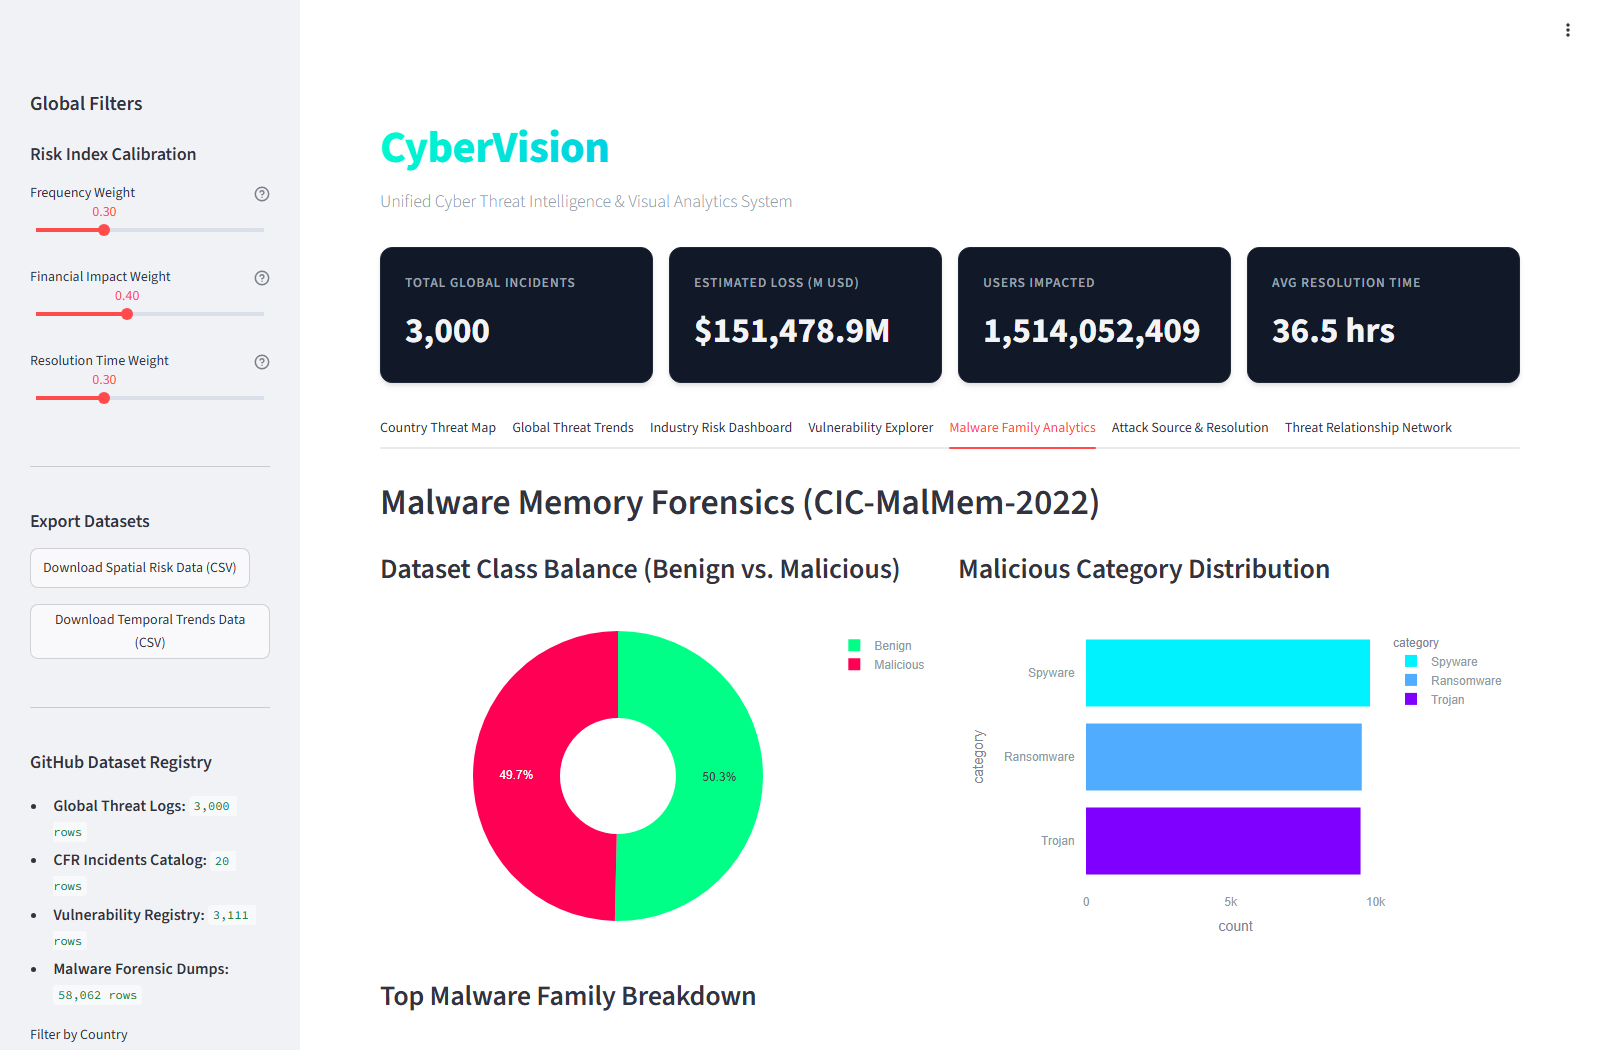
\includegraphics[width=0.85\textwidth]{images/malware_analytics.png}
    \caption{Malware family memory classification distribution.}
    \label{fig:malware}
\end{figure}

\subsection{Threat Attribution and Resolution Efficiency}
We correlate threat actor types (Hackers, Nation-States, Insiders) and defense controls with operational containment times using an interactive scatter plot. The plot displays a dense distribution of resolution times spanning from immediate containment up to 70 hours. Crucially, no single defense mechanism (VPN, Antivirus, AI detection, or Firewalls) emerges as a single silver bullet that guarantees fast resolution. Instead, we observe significant overlap across all controls. Furthermore, Advanced Persistent Threats (APTs) launched by nation-states exhibit long, persistent lifecycles that require extensive audit and forensics. This shows that containment time is driven not just by the tool deployed, but by the sophistication of the attacker, necessitating a defense-in-depth posture.

\begin{figure}[h!]
    \centering
    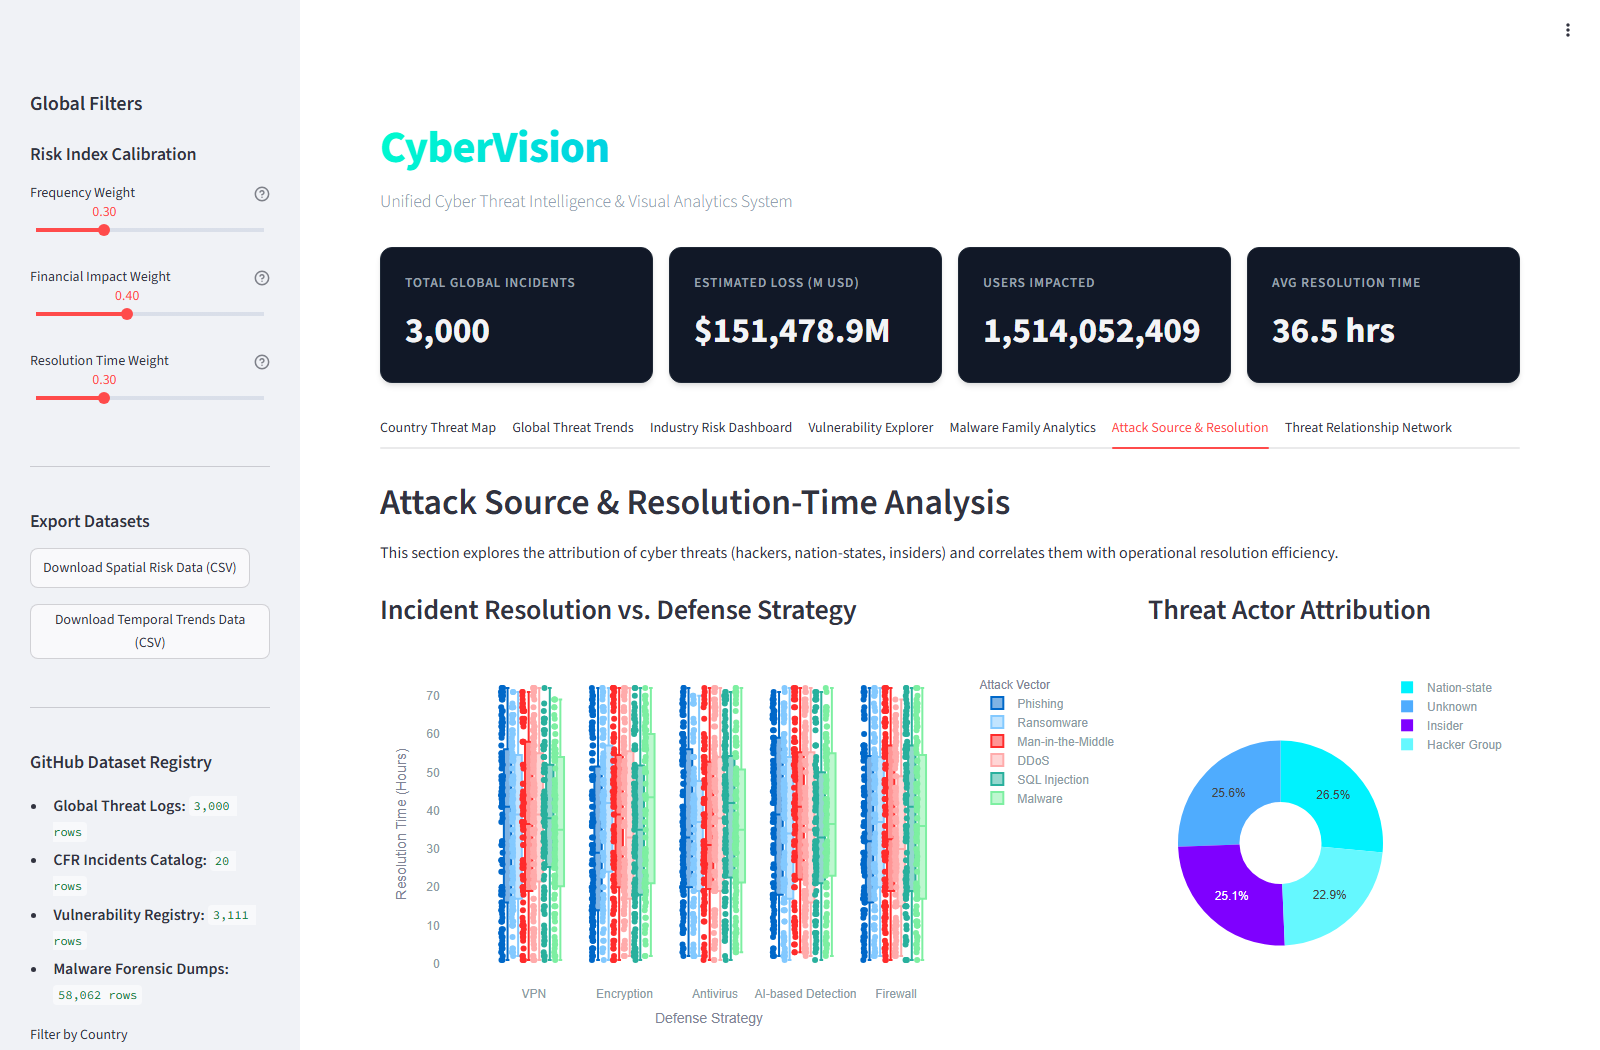
\includegraphics[width=0.85\textwidth]{images/attack_source.png}
    \caption{Box plots of incident resolution times grouped by defense mechanism.}
    \label{fig:resolution}
\end{figure}

\subsection{Geopolitical Relationship Network}
The complex relationship paths connecting threat sources, target countries, and target commercial sectors are mapped using a force-directed spring graph. To prevent visual clutter while preserving rich insights, we implemented a 3-tier weighted edge system. Weak links (Frequency=1) are rendered as thin, low-opacity lines (0.08) to show isolated alerts, while Strong links (Frequency>3) are represented as thick, pink traces. The graph reveals high connectivity clusters centering on nation-state actors targeting critical infrastructure and finance hubs in North America and Western Europe. This visual clustering shows that state-sponsored actors concentrate their resources on high-value geopolitical targets rather than dispersing attacks, highlighting the target profiles of modern cyber warfare.

\begin{figure}[h!]
    \centering
    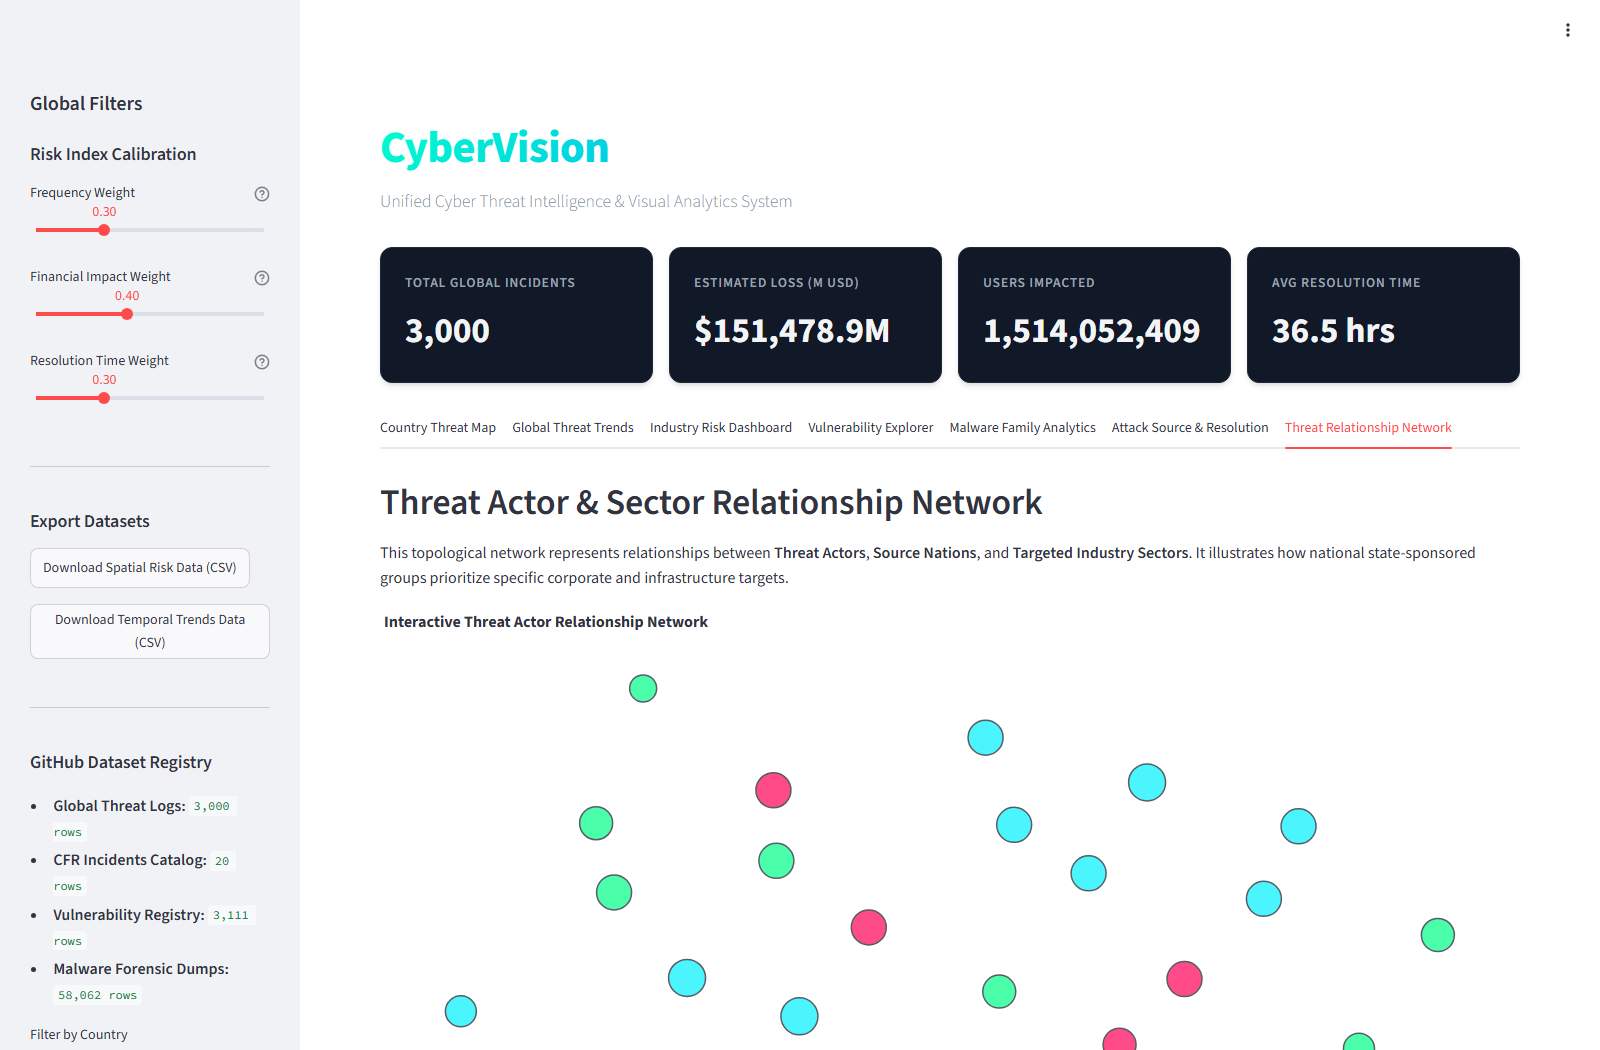
\includegraphics[width=0.85\textwidth]{images/threat_network.png}
    \caption{Threat Relationship Network mapping connections between threat vectors and sectors.}
    \label{fig:network}
\end{figure}

% ----------------- CHAPTER 5: RESULTS AND FINDINGS -----------------
\chapter{Results and Findings}
CyberVision provides structured, quantitative findings derived directly from the integrated data.

\subsection{Country Risk Leaderboard}
Aggregated results from \texttt{integrated\_spatial.csv} show the national risk indices calculated under standard weights ($w\_{\text{freq}} = 0.3, w\_{\text{loss}} = 0.4, w\_{\text{time}} = 0.3$).

\begin{table}[h!]
\centering
\small
\caption{National Threat Risk Leaderboard}
\begin{tabular}{cccccc}
\toprule
\textbf{Rank} & \textbf{Country} & \textbf{Incidents} & \textbf{Total Loss (\$M)} & \textbf{Avg. Resolution (hrs)} & \textbf{Risk Score} \\
\midrule
1 & United Kingdom & 321 & 15,746.49 & 37.1 & 7.68 \\
2 & Brazil & 310 & 16,880.70 & 36.8 & 6.97 \\
3 & Germany & 291 & 14,767.36 & 37.5 & 5.58 \\
4 & Japan & 305 & 14,871.81 & 36.4 & 5.31 \\
5 & Australia & 297 & 15,403.00 & 36.5 & 5.18 \\
6 & France & 305 & 15,622.91 & 36.0 & 4.17 \\
7 & India & 308 & 14,917.87 & 35.8 & 3.21 \\
8 & Russia & 295 & 15,219.18 & 35.7 & 3.11 \\
9 & United States & 287 & 14,420.09 & 36.2 & 3.07 \\
10 & China & 281 & 13,958.09 & 35.8 & 2.57 \\
\bottomrule
\end{tabular}
\end{table}

\subsection{Industry Sector Loss Projections}
Summarized sector distributions expose which industries bear the largest financial burdens:
\begin{itemize}
    \item \textbf{IT Infrastructure:} Registers the highest average financial loss per incident (\$51.2M), indicating that IT services are highly leveraged targets.
    \item \textbf{Healthcare:} Records the largest aggregate financial loss (\$21,804M), reflecting high compliance and remediation costs.
    \item \textbf{Banking \& Financial Services:} Follows closely with a total loss of \$21,120M, driven by direct theft targets.
\end{itemize}

\subsection{Network Traffic Protocol Share}
From the analysis of 40,000 traffic records in \texttt{attack\_signatures\_clean.csv}, the distribution of network protocols is:
\begin{itemize}
    \item \textbf{ICMP (Internet Control Message Protocol):} 13,429 records (33.57\% share) --- typically associated with ping sweeps and denial-of-service amplification.
    \item \textbf{UDP (User Datagram Protocol):} 13,299 records (33.25\% share) --- indicating high-volume traffic flooding attacks.
    \item \textbf{TCP (Transmission Control Protocol):} 13,272 records (33.18\% share) --- representing standard connection-oriented exploit payloads.
\end{itemize}

\subsection{Vulnerability Severity Breakdown}
The distribution of the 3,111 software vulnerabilities published between 2021 and 2023 is:
\begin{itemize}
    \item \textbf{Moderate Severity:} 1,447 CVEs (46.51\%)
    \item \textbf{High Severity:} 1,048 CVEs (33.68\%)
    \item \textbf{Critical Severity:} 449 CVEs (14.43\%)
    \item \textbf{Low Severity:} 167 CVEs (5.38\%)
\end{itemize}

% ----------------- CHAPTER 6: DISCUSSION -----------------
\chapter{Discussion}

\subsection{Geopolitical and Economic Risk Dynamics}
The country risk leaderboard indicates that cyber risk is not a direct reflection of a country's size or population. While the United Kingdom and Brazil occupy the top ranks, the United States and China exhibit lower scores. This pattern is driven by the components of the Country Risk Index:
\begin{itemize}
    \item Brazil exhibits the highest total financial loss (\$16,880.70M), indicating a lack of robust security controls.
    \item The UK reports the highest number of incidents (321) and a high average resolution time (37.1 hours), reflecting active targeting and regulatory reporting requirements.
    \item The US and China exhibit lower average resolution times and lower reported average financial losses per incident in this dataset, which drags down their normalized risk scores.
\end{itemize}
It is worth stressing that this ranking is a function of the \textit{reported} data and the chosen weighting scheme, not an absolute measure of national cybersecurity maturity; a jurisdiction with stricter incident-disclosure requirements will mechanically report more incidents than one without such requirements, independent of its true underlying exposure.

\subsection{Vulnerability Lifecycle and Threat Landscape Shift}
The CVE severity distribution highlights a shift in threat dynamics. The concentration of High and Critical vulnerabilities in 2023 suggests that software development lifecycles struggle to secure complex, cloud-native deployments. The lag in patch deployment allows threat actors to exploit vulnerabilities before organizations can apply updates, which is consistent with the broader industry observation that the median time-to-patch for critical vulnerabilities routinely exceeds the time-to-exploit once a proof-of-concept is public.

\subsection{Practical Significance and Cyber Defense Tactics}
The findings of CyberVision have practical implications for security operations:
\begin{enumerate}
    \item \textbf{Dynamic Risk Alignment:} Organizations must calibrate security budgets to match their risk profiles (e.g. financial damage vs. operational uptime).
    \item \textbf{Memory Forensic Deployment:} Endpoint detection tools must incorporate machine learning models capable of analyzing high-dimensional memory structures to identify obfuscated malware processes.
    \item \textbf{Deep Packet Filtering:} Firewalls must inspect large packets, which are strongly correlated with anomalous traffic signatures.
\end{enumerate}

\subsection{Limitations of the Analysis}
\begin{itemize}
    \item \textbf{Static Weights:} Although user-adjustable in the UI, default weights in the backend code are hardcoded.
    \item \textbf{Geographic Representation:} Standardization maps geographic data to ten standard industrial nations, which limits the analysis of emerging markets.
    \item \textbf{Volatile Features:} The memory forensic dataset uses features specific to Volatility 2, which may not capture memory structures in modern operating systems.
\end{itemize}

% ----------------- CHAPTER 7: CHALLENGES -----------------
\chapter{Challenges}

\subsection{High-Dimensional Volatility Memory Forensics}
The MalMem dataset presents a classic ``curse of dimensionality'' challenge, containing 58 features representing process list states, loaded DLLs, and open handles. Visualizing these features in a 2D dashboard requires aggregation or dimensionality reduction (e.g. PCA), which can mask subtle indicators of malicious activity. Selecting which handful of derived dimensions to surface on a dashboard, without discarding the signal that a forensic analyst would actually need, proved to be one of the more delicate design trade-offs in the project.

\subsection{Data Inconsistencies and Missing Value Imputations}
Ingesting multiple CTI datasets introduces inconsistencies:
\begin{itemize}
    \item Timestamps use varying formats, requiring robust date parsing routines.
    \item Missing categorical attributes require imputation to prevent data loss. Filling missing fields with ``Unknown'' preserves sample sizes but can introduce noise into categorical aggregations.
\end{itemize}

\subsection{Network Graph Scaling and Layout Constraints}
Visualizing the Geopolitical Relationship Network using NetworkX and Plotly introduces layout challenges. Projects with over 150 nodes suffer from overlapping nodes and visual clutter, reducing the legibility of threat actor paths. The static spring-layout algorithm lacks interactive physics, making it difficult to trace complex networks, and was ultimately one of the motivating factors behind the physics-based rendering proposed in Section 9.3.

% ----------------- CHAPTER 8: CONCLUSION -----------------
\chapter{Conclusion}

\subsection{Summary of Accomplished Objectives}
\begin{itemize}
    \item Designed and verified a reproducible data cleaning and integration pipeline.
    \item Developed a dynamic Country and Industry Risk Index using Min--Max scaling.
    \item Implemented high-contrast, neon-colored visualizations to analyze threat trends, network forensics, and memory states.
    \item Created a cached, multi-page Streamlit dashboard featuring a modern glassmorphic theme.
\end{itemize}

\subsection{Key Analytical Insights}
\begin{itemize}
    \item Peak attack periods correlate with global security events (e.g. ransomware outbreaks in 2017, geopolitical tensions in 2022).
    \item Highly digitized, service-oriented economies exhibit higher reported risk indices.
    \item Network traffic analysis shows a strong correlation between large packet lengths and high anomaly scores, indicating payload-based exploits.
\end{itemize}

\subsection{Platform Success and Practical Utility}
CyberVision demonstrates the value of interactive big data visualization in security operations. By unifying disparate telemetry feeds, the platform reduces cognitive load and alert fatigue, enabling security analysts to make data-driven defensive decisions rather than manually reconciling isolated tools and spreadsheets.

% ----------------- CHAPTER 9: FUTURE SCOPE -----------------
\chapter{Future Scope}

\subsection{Predictive Alerting Engines and Time-Series Forecasting}
A logical next step for CyberVision is the integration of predictive engines. Incorporating forecasting models (e.g. Prophet or ARIMA) would enable the platform to project future incident volumes based on historical trends, helping organizations allocate security resources proactively rather than reactively.

\subsection{Integration of Standard CVSS Severity in Country Risk Calculations}
To improve the Country Risk Index, future versions should incorporate CVSS (Common Vulnerability Scoring System) severity levels. Weighting incidents by vulnerability severity would provide a more accurate representation of risk than simple incident counts, since two countries with identical incident counts may face very different underlying exposure if one set of incidents involves critical remote-code-execution vulnerabilities and the other does not.

\subsection{Interactive Physics-Based Graph Renderings}
Replacing static NetworkX/Plotly network graphs with physics-based, interactive libraries (e.g. Pyvis or D3.js) would enhance usability. Dynamic layouts would resolve node overlap and allow analysts to manipulate nodes to inspect threat paths, directly addressing the scaling constraints identified in Section 7.3.

\subsection{Cloud Deployment and Real-Time Stream Integration}
Deploying CyberVision to cloud platforms (e.g., AWS, GCP) and integrating real-time message brokers (e.g. Apache Kafka) would transform the dashboard from a batch-oriented analytics tool into a real-time monitoring system, capable of ingesting and visualizing telemetry as it arrives rather than on a periodic refresh cycle.

\newpage
% ----------------- CODE AND DEPLOYMENT LINKS -----------------
\chapter{Code and Deployment Links}
\begin{itemize}
    \item \textbf{GitHub Repository (Group):} \href{https://github.com/haryashva/Cyber-Attach-Visualisation}{github.com/haryashva/Cyber-Attach-Visualisation}
    \item \textbf{GitHub Repository (Fork):} \href{https://github.com/nikitanehrag24-a11y/Cyber-Attach-Visualisation}{github.com/nikitanehrag24-a11y/Cyber-Attach-Visualisation}
    \item \textbf{Live Deployed Web Application:} \href{https://cyber-attach-visualisation-dawavmaacerhnvodttg9rb.streamlit.app/}{cyber-attach-visualisation.streamlit.app}
\end{itemize}

\bibliographystyle{unsrt}
\bibliography{references}

\newpage
\appendix
\chapter{Appendices}

\section{Complete Repository Folder Structure}
\_\_LST\_BLOCK\_0\_\_

\section{Software and Package Requirements}
The system requires Python 3.9+ and the packages listed in \texttt{requirements.txt}:
\_\_LST\_BLOCK\_1\_\_

\section{Environment Setup and Execution Guide}
To deploy CyberVision locally:
\begin{enumerate}
    \item Clone the repository:
    \_\_LST\_BLOCK\_2\_\_
    \item Create and activate a virtual environment:
    \_\_LST\_BLOCK\_3\_\_
    \item Install dependencies:
    \_\_LST\_BLOCK\_4\_\_
    \item Acquire the datasets:
    \begin{itemize}
        \item Set up Kaggle API credentials (\texttt{\~{}/.kaggle/kaggle.json}).
        \item Run the automated download script:
        \_\_LST\_BLOCK\_5\_\_
        \item Manually download \texttt{cic\_malmem\_2022.csv} from the UNB portal and place it in \texttt{data/raw/}.
    \end{itemize}
    \item Run the cleaning and integration pipelines:
    \_\_LST\_BLOCK\_6\_\_
    \item Launch the Streamlit web application:
    \_\_LST\_BLOCK\_7\_\_
    Open \url{http://localhost:8501} in your web browser.
\end{enumerate}

\section{Important Preprocessing \& Risk Logic Snippets}

\_\_LST\_BLOCK\_8\_\_

\_\_LST\_BLOCK\_9\_\_

\end{document}